\documentclass{beamer}
\usepackage{ctex}
\usepackage{hyperref}
\usepackage[T1]{fontenc}
\usepackage{amssymb}
\usepackage{relsize}
\usepackage{multicol}
\usepackage{subcaption} 

% other packages
\usepackage{latexsym,amsmath,xcolor,multicol,booktabs,calligra}
\usepackage{graphicx,pstricks,listings,stackengine}

\title{数理统计中的三大分布及其应用}
\subtitle{The Three Major Distributions in Mathematical Statistics\\ and their Applications}
% 【已修改】：将真实姓名和导师姓名替换为通用占位符
\author[Presenter]{Applicant \and Academic Advisor}
\institute{上海理工大学基础学部 数学学院}
\date{2026年5月26日}

% new defs
\def\cmd#1{\texttt{\color{red}\footnotesize $\backslash$#1}}
\def\env#1{\texttt{\color{blue}\footnotesize #1}}
\definecolor{deepblue}{rgb}{0,0,0.5}
\definecolor{deepred}{rgb}{0.6,0,0}
\definecolor{deepgreen}{rgb}{0,0.5,0}
\definecolor{halfgray}{gray}{0.55}

% 无标题的block框
\newenvironment{block*}
  {\setbeamercolor{block title}{bg=white,fg=white}%
   \begin{block}{}}
  {\end{block}}
%---------------------------------------------------------------------

% beamer 主题
\usetheme{AnnArbor}
\usecolortheme{beaver}
\setbeamertemplate{blocks}[rounded][shadow=true]

% beamer 命令框
\setbeamercolor{block body}{bg=structure!10}
\setbeamercolor{block title}{bg=structure!20}

% 图片自动编号
\setbeamertemplate{caption}[numbered]

% 每个frame的下框
\makeatletter
\setbeamertemplate{footline}
{
  \leavevmode%
  \hbox{%
    \begin{beamercolorbox}[wd=.155\paperwidth,ht=2.5ex,dp=1.125ex,center]{author in head/foot}%
      \usebeamerfont{author in head/foot}\insertshortauthor
    \end{beamercolorbox}%
    \begin{beamercolorbox}[wd=.58\paperwidth,ht=2.5ex,dp=1.125ex,center]{title in head/foot}%
      \usebeamerfont{title in head/foot}\insertshorttitle
    \end{beamercolorbox}%
    \begin{beamercolorbox}
    [wd=.265\paperwidth,ht=2.5ex,dp=1.125ex,right]{date in head/foot}%
      \usebeamerfont{date in head/foot}
      \insertshortdate{} \hspace{1em}
      \usebeamerfont{frame number}\insertframenumber/\inserttotalframenumber\hspace{1em}
    \end{beamercolorbox}%
  }%
  \vskip0pt%
}
\makeatother

% 新颜色
\xdefinecolor{usst}{RGB}{154,3,0}  
\setbeamercolor{title}{bg=usst,fg=white}

% 每页右下角乱七八糟的标识
\setbeamertemplate{navigation symbols}{}

% 进入章节目录
\AtBeginSection[]{
	\begin{frame}
		\tableofcontents[sectionstyle=show/shaded,subsectionstyle=show/shaded/hide,subsubsectionstyle=show/shaded/hide]
	\end{frame}
}

\AtBeginSubsection[]{
	\begin{frame}
		\tableofcontents[sectionstyle=show/shaded,subsectionstyle=show/shaded/hide,subsubsectionstyle=show/shaded/hide]
	\end{frame}
}

% 理学院背景
\setbeamertemplate{background}{
\includegraphics[width=12.8cm]{pic/background-理学院-2.pdf}}


%---------------------------------------------------------------------

\begin{document}
\kaishu

% 封面页
\begin{frame}
    \titlepage
    \begin{figure}[htpb]
        \begin{center}
            
\includegraphics[width=0.4\linewidth]{pic/USST_logo.eps}
        \end{center}
    \end{figure}
\end{frame}

% 目录页
\begin{frame}
    \tableofcontents[sectionstyle=show,subsectionstyle=show/shaded/hide,subsubsectionstyle=show/shaded/hide]
\end{frame}


%=====================================================================
% 第一章：引言
%=====================================================================

\section{引言}

% 1.1 研究背景（1页）
\subsection{研究背景}
\begin{frame}{研究背景}
    \begin{block}{三大分布的重要性}
        数理统计中的三大分布——\(\chi^2\)分布、\(t\)分布和\(F\)分布是参数估计与假设检验的理论基石。它们共同构成了统计推断的核心框架，在医学、经济、教育等多个领域广泛应用。
    \end{block}

    \vspace{0.3cm}

    \begin{block*}
        统计分布既是数据分析的概率模型，又是统计的基石，在任何一个统计分布模型中几乎都有应用。
    \end{block*}
\end{frame}

% 1.2 研究现状（2页）
\subsection{研究现状}
\begin{frame}{理论层面研究现状}
    \begin{block}{基础理论}
        \begin{itemize}
            \item 刘晓鹏与刘坤会（2005）：详细分析了\(F\)分布密度函数与参数之间的关系
            \item 陈浩明（2008）：贝叶斯框架下的后验分布研究
            \item Azzalini与Dalla Valle（1996）：多元偏态正态分布族
        \end{itemize}
    \end{block}

    \vspace{0.3cm}

    \begin{block}{多元推广}
        \begin{itemize}
            \item 江忠伟（2016）：似然比法导出霍特林\(T^2\)分布与威尔克斯\(\Lambda\)分布
            \item Lange等（2023）：\(t\)分布在稳健统计建模中的优势
            \item Nadarajah与Kotz（2020）：多元\(t\)分布估计方法综述
        \end{itemize}
    \end{block}
\end{frame}

\begin{frame}{应用层面研究现状}
    \begin{block}{医学与生物领域}
        \begin{itemize}
            \item 卢文丽等（2002）：霍特林\(T^2\)检验及MANOVA应用于生存质量资料分析
            \item 黄卓慧（2026）：采用MANOVA分析神经影像数据
            \item Arroyo等（2025）：验证狨猴体况评分能预测体重和身体组成
        \end{itemize}
    \end{block}

    \vspace{0.3cm}

    \begin{block}{社会科学领域}
        \begin{itemize}
            \item 赵雅娟（2025）：采用配对\(t\)检验和MANOVA分析初中生学习动机
            \item 张小平（2025）：运用\(t\)检验、方差分析研究硕士研究生就业能力
        \end{itemize}
    \end{block}
\end{frame}


%=====================================================================
% 第二章：理论基础
%=====================================================================

\section{理论基础}

% 2.1 卡方分布（1页）
\subsection{\(\chi^2\)分布}
\begin{frame}{\(\chi^2\)分布}
    \begin{block}{定义}
        设 \(X_1, X_2, \cdots, X_n\) 独立同分布于标准正态分布 \(N(0, 1)\)，记
        \[\chi^2 = X_1^2 + X_2^2 + \cdots + X_n^2\]
        则称 \(\chi^2\) 服从自由度为 \(n\) 的 \(\chi^2\) 分布，记为 \(\chi^2 \sim \chi^2(n)\)。
    \end{block}

    \vspace{0.3cm}

    \begin{block}{主要性质}
        \begin{itemize}
            \item 期望：\(E(\chi^2) = n\)
            \item 方差：\(Var(\chi^2) = 2n\)
            \item 可加性：若\(\chi_1^2 \sim \chi^2(n_1)\)，\(\chi_2^2 \sim \chi^2(n_2)\)且相互独立，则\(\chi_1^2 + \chi_2^2 \sim \chi^2(n_1+n_2)\)
        \end{itemize}
    \end{block}
\end{frame}

% 2.2 t分布（1页）
\subsection{\(t\)分布}
\begin{frame}{\(t\)分布}
    \begin{block}{定义}
        设随机变量 \(X\) 与 \(Y\) 相互独立，且 \(X \sim N(0,1)\)，\(Y \sim \chi^2(n)\)，则称
        \[t = \frac{X}{\sqrt{Y/n}}\]
        服从自由度为 \(n\) 的 \(t\) 分布，记为 \(t \sim t(n)\)。
    \end{block}

    \vspace{0.3cm}

    \begin{block}{主要性质}
        \begin{itemize}
            \item 期望：\(E(t) = 0\)（当\(n>1\)时）
            \item 方差：\(Var(t) = \frac{n}{n-2}\)（当\(n>2\)时）
        \end{itemize}
    \end{block}
\end{frame}

% 2.3 F分布（1页）
\subsection{\(F\)分布}
\begin{frame}{\(F\)分布}
    \begin{block}{定义}
        设随机变量 \( X \sim \chi^2(n_1) \), \( Y \sim \chi^2(n_2) \)，\( X \) 与 \( Y \) 相互独立，则称
        \[F = \frac{X/n_1}{Y/n_2}\]
        服从自由度为 \((n_1, n_2)\) 的 \( F \) 分布，记为 \( F \sim F(n_1, n_2) \)。
    \end{block}

    \vspace{0.3cm}

    \begin{block}{主要性质}
        \begin{itemize}
            \item 若\(F \sim F(n_1, n_2)\)，则\(1/F \sim F(n_2, n_1)\)
            \item 若\(X \sim t(n)\)，则\(X^2 \sim F(1, n)\)
            \item 在大样本下，当\( n_2 \to \infty \) 时，\[\mathbf{n}_1 \mathbf{F} \xrightarrow{\mathbf{d}} \chi^2(\mathbf{n}_1)\]
        \end{itemize}
    \end{block}
\end{frame}

% 2.4 三大分布的内在联系（1页）
\subsection{三大分布的内在联系}
\begin{frame}{三大分布的内在联系}
    \begin{block}{衍生关系}
        \begin{itemize}
            \item \(\chi^2\)分布源于正态变量的平方和
            \item \(t\)分布由正态变量与\(\chi^2\)分布构造
            \item \(F\)分布由两个独立\(\chi^2\)分布之比构成
        \end{itemize}
    \end{block}

    \vspace{0.5cm}

    \begin{alertblock}{重要结论}
        \(t\)分布的平方服从第一自由度为1的\(F\)分布：
        \[t^2 \sim F(1, n)\]
    \end{alertblock}

    \vspace{0.5cm}

    \begin{block*}
        三大分布共同构成了统计推断的底层框架，体现了方法的统一性和连贯性。
    \end{block*}
\end{frame}


%=====================================================================
% 第三章：数据与方法
%=====================================================================

\section{数据与方法}

% 3.1 数据来源（1页）
\subsection{数据来源}
\begin{frame}{数据来源}
    \begin{block}{数据集介绍}
        \begin{itemize}
            \item 来源：Kaggle学生学业表现数据集
            \item 样本量：6607条学生记录
            \item 变量：11个特征变量
        \end{itemize}
    \end{block}

    \vspace{0.5cm}

    \begin{block}{变量说明}
        \begin{columns}
            \column{0.45\textwidth}
            \begin{block}{自变量}
                \begin{itemize}
                    \item 网络接入（二分类）
                    \item 课外活动（二分类）
                    \item 父母参与度（三分类）
                \end{itemize}
            \end{block}
            
            \column{0.45\textwidth}
            \begin{block}{因变量}
                \begin{itemize}
                    \item 最终考试成绩
                    \item 出勤率
                    \item 学习时长
                \end{itemize}
            \end{block}
        \end{columns}
    \end{block}

    \vspace{0.5cm}

    \begin{alertblock}{研究设计}
        本研究采用单变量与多元分析相结合的方法，全面评估各因素对学生学业表现的影响
    \end{alertblock}
\end{frame}

% 3.2 数据预处理
\subsection{数据预处理}
% 3.2.1 缺失值与异常值（文字说明）
\begin{frame}{数据预处理：缺失值与异常值}
    \begin{block}{缺失值处理}
        \begin{itemize}
            \item 经检查，数据集各变量均无缺失值
            \item 无需进行缺失值填补或删除操作
        \end{itemize}
    \end{block}

    \vspace{0.3cm}

    \begin{block}{异常值检测}
        \begin{itemize}
            \item 采用箱线图法对各连续变量进行检测
            \item Hours\_Studied：18个离群点（0.27\%）
            \item Final\_Exam\_Score：10个离群点（0.15\%）
            \item 离群点均在合理取值范围内，予以保留
        \end{itemize}
    \end{block}
\end{frame}

% 3.2.2 箱线图
\begin{frame}{异常值检测：箱线图分布}
    \centering
    \begin{figure}
        % 第一行：3张图，每张占30%宽度
        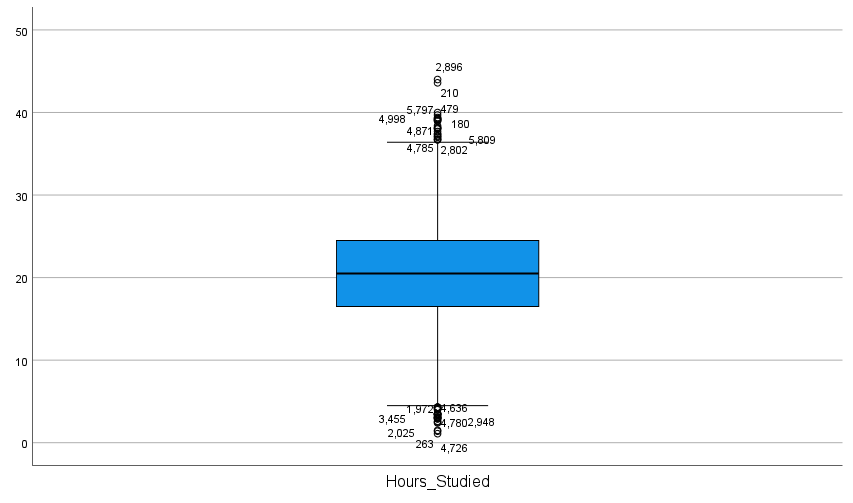
\includegraphics[width=0.3\linewidth]{pic/图3.1 Hours_Studied的箱线图.png}
        \hspace{0.3cm}
        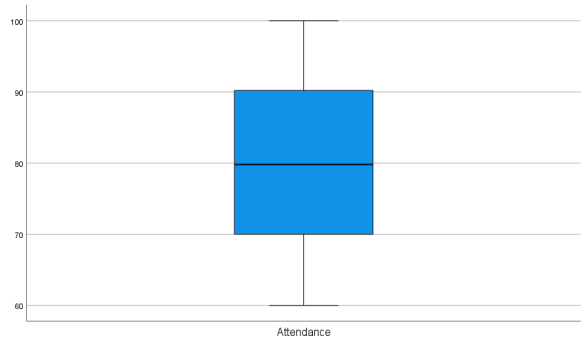
\includegraphics[width=0.3\linewidth]{pic/图3.2 Attendance的箱线图.png}
        \hspace{0.3cm}
        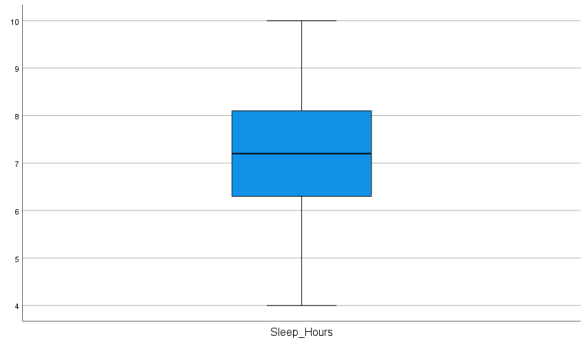
\includegraphics[width=0.3\linewidth]{pic/图3.3 Sleep_Hours的箱线图.png}
        
        \vspace{0.4cm}
        
        % 第二行：2张图，每张占30%宽度，居中显示
        \hspace*{\fill}
        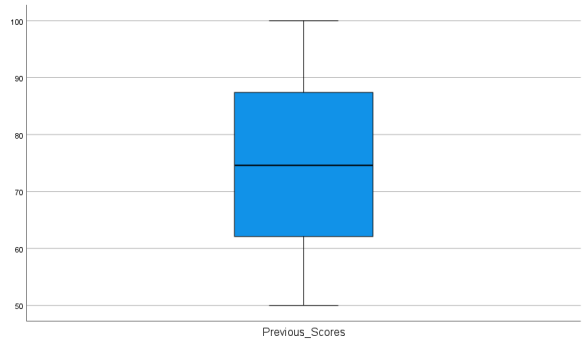
\includegraphics[width=0.3\linewidth]{pic/图3.4 Previous_Scores的箱线图.png}
        \hspace{0.3cm}
        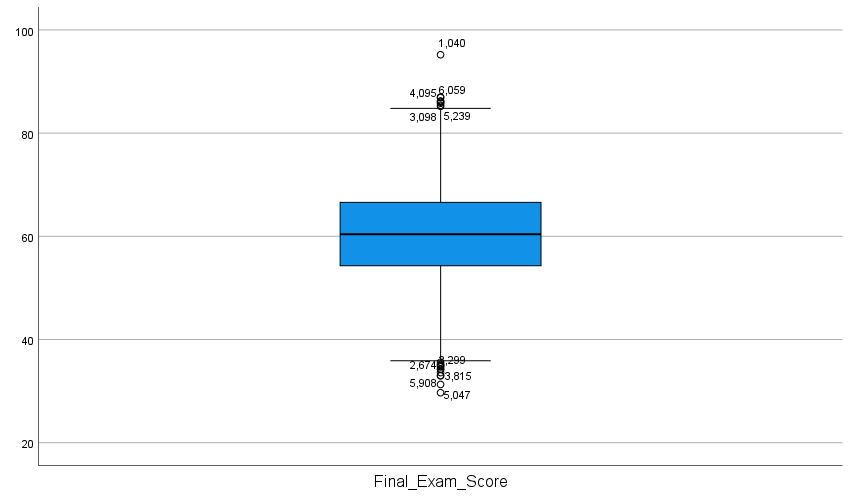
\includegraphics[width=0.3\linewidth]{pic/图3.5 Final_Exam_Score的箱线图.png}
        \hspace*{\fill}
        \caption{各变量箱线图分布}
    \end{figure}
\end{frame}

% 3.2.3 正态性检验
\subsection{正态性检验}
% Q-Q图（4张图）
\begin{frame}{正态性检验：Q-Q图分布}
    \centering
    \begin{figure}
        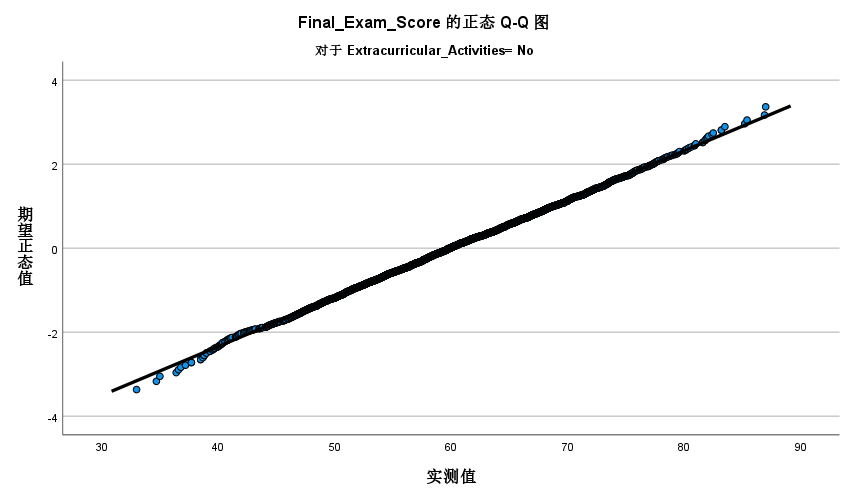
\includegraphics[width=0.3\linewidth]{pic/图3.10 未参加课外活动组Q-Q图.png}
        \hspace{0.3cm}
        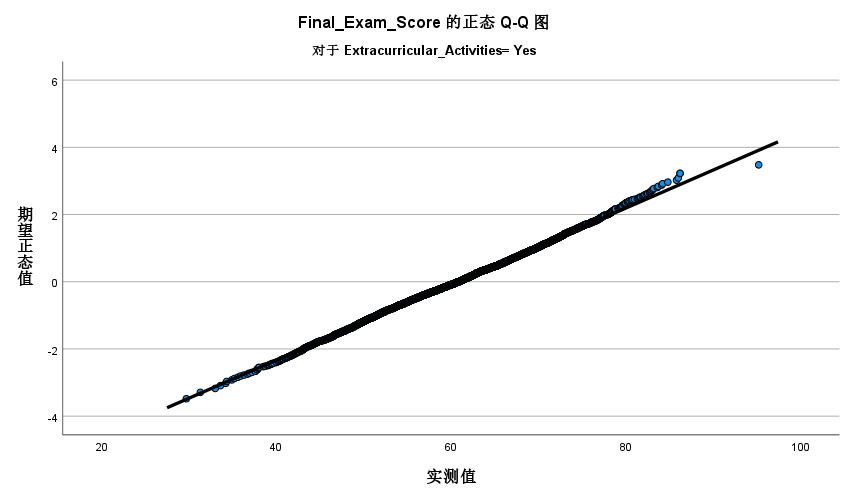
\includegraphics[width=0.3\linewidth]{pic/图3.11 参加课外活动组Q-Q图.png}
        \hspace{0.3cm}
        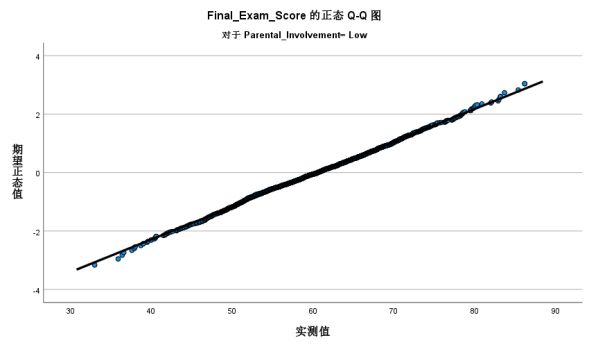
\includegraphics[width=0.3\linewidth]{pic/图3.12 父母参与度低组Q-Q图.png}
        
        \vspace{0.3cm}
        
        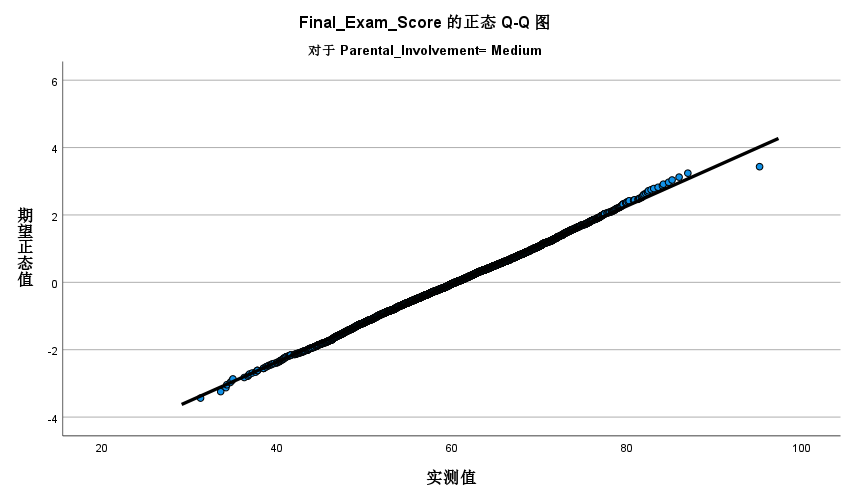
\includegraphics[width=0.3\linewidth]{pic/图3.13 父母参与度中组Q-Q图.png}
        \hspace{0.3cm}
        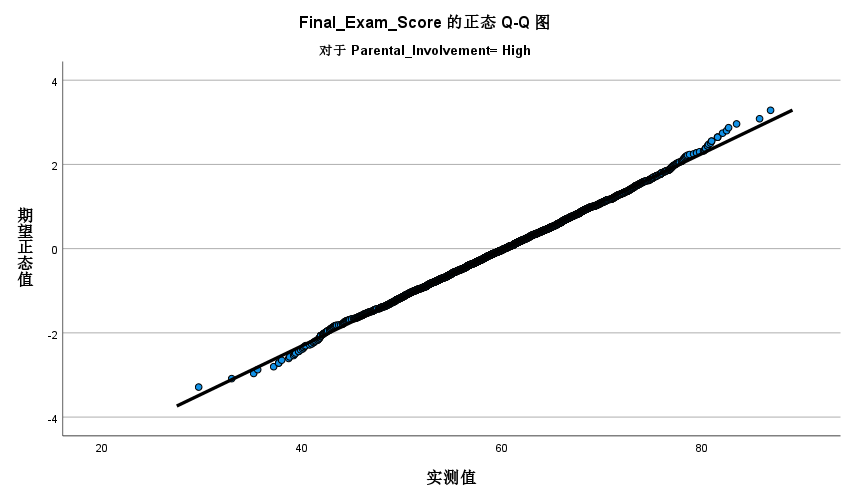
\includegraphics[width=0.3\linewidth]{pic/图3.14 父母参与度高组Q-Q图.png}
        \caption{各分组Q-Q图正态性检验}
    \end{figure}
\end{frame}

% 直方图（5张图）
\begin{frame}{正态性检验：成绩分布直方图}
    \centering
    \begin{figure}
        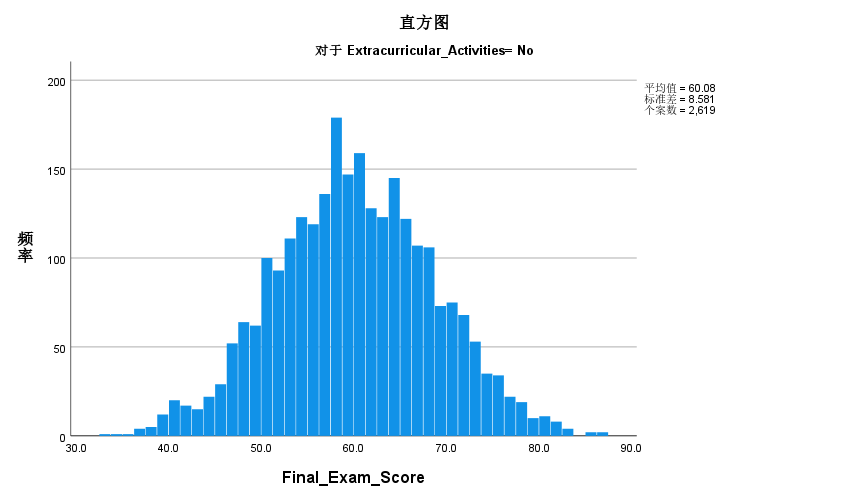
\includegraphics[width=0.3\linewidth]{pic/图3.15 未参与课外活动组直方图.png}
        \hspace{0.3cm}
        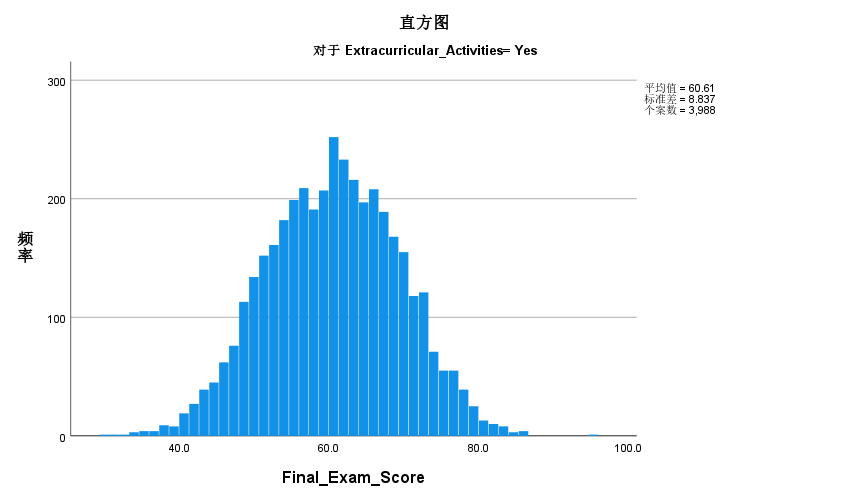
\includegraphics[width=0.3\linewidth]{pic/图3.16 参与课外活动组直方图.png}
        \hspace{0.3cm}
        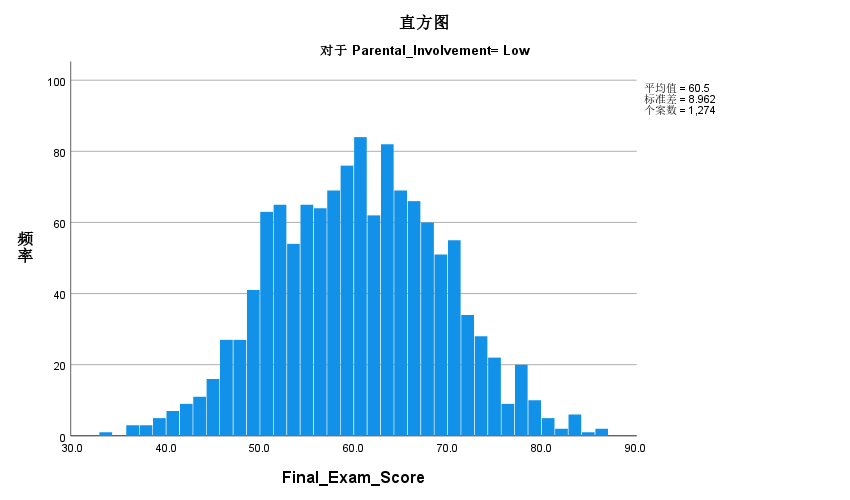
\includegraphics[width=0.3\linewidth]{pic/图3.17 父母参与度低组直方图.png}
        
        \vspace{0.3cm}
        
        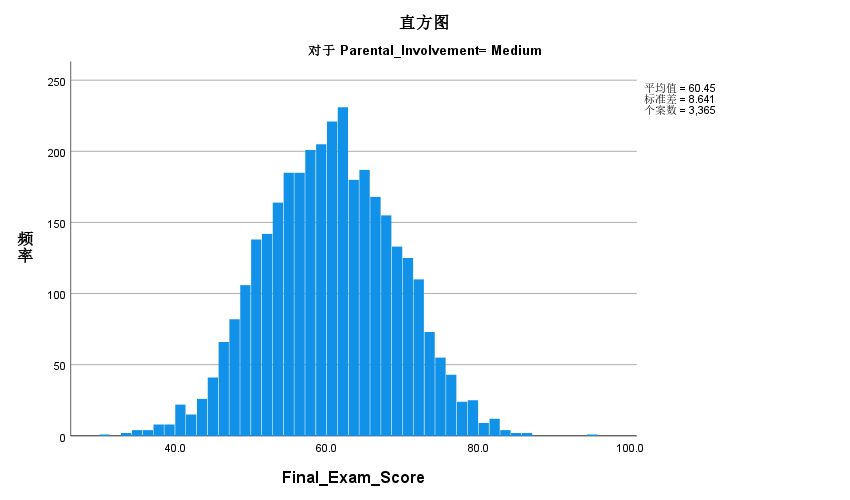
\includegraphics[width=0.3\linewidth]{pic/图3.18 父母参与度中组直方图.png}
        \hspace{0.3cm}
        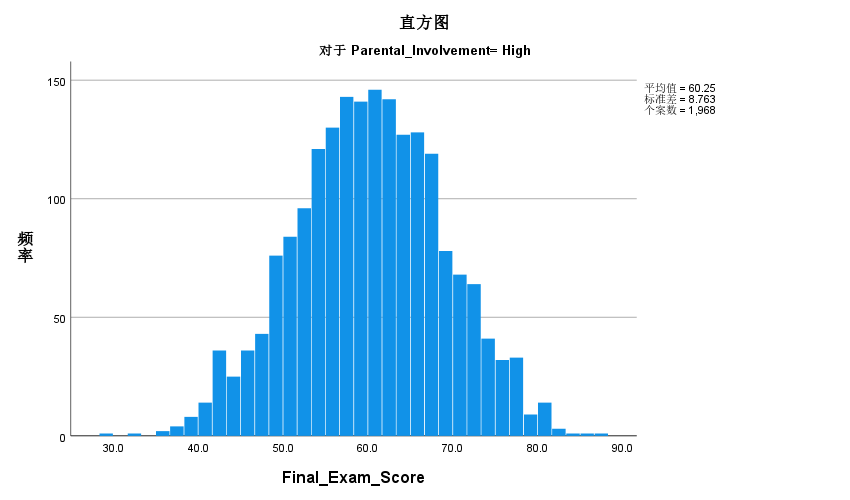
\includegraphics[width=0.3\linewidth]{pic/图3.19 父母参与度高组直方图.png}
        \caption{各分组成绩分布直方图}
    \end{figure}
\end{frame}

% 3.2.4 描述性统计与结论
\begin{frame}{描述性统计与结论}
    \begin{block}{描述性统计}
        最终考试成绩的基本统计特征：
        \begin{itemize}
            \item 平均分：60.4分
            \item 标准差：8.739
            \item 偏度：0.017（近似正态）
            \item 峰度：-0.212（略偏扁平）
        \end{itemize}
    \end{block}

    \vspace{0.5cm}

    \begin{alertblock}{数据质量结论}
        数据满足参数检验的基本假设，包括正态性、独立性和方差齐性，可进行后续的单变量和多元分析。
    \end{alertblock}
\end{frame}




%=====================================================================
% 第四章：单变量实证
%=====================================================================

\section{单变量实证}

% 4.1 卡方检验（2页）
\subsection{\(\chi^2\)检验}
\begin{frame}{4.1 \(\chi^2\)检验：研究问题与数据}
    \begin{block}{研究问题}
        学生的网络接入情况与是否及格是否存在关联？
    \end{block}

    \vspace{0.3cm}

    \begin{table}
        \centering
        \renewcommand{\arraystretch}{1.3}
        \begin{tabular}{lccc}
            \toprule
            & 不及格 & 及格 & 合计 \\
            \midrule
            无网络 & 257 & 257 & 514 \\
            有网络 & 2903 & 3190 & 6093 \\
            合计 & 3160 & 3447 & 6607 \\
            \bottomrule
        \end{tabular}
        \caption{网络接入与及格情况列联表}
    \end{table}
\end{frame}

\begin{frame}{4.1 \(\chi^2\)检验：结果与结论}
    \begin{block}{检验结果}
        \begin{itemize}
            \item \(\chi^2 = 1.054\)
            \item 自由度 \(df = 1\)
            \item \(p= 0.305 > 0.05\)
        \end{itemize}
    \end{block}

    \vspace{0.5cm}

    \begin{alertblock}{结论}
        网络接入情况与最终考试及格情况无显著关联，未拒绝原假设。
    \end{alertblock}

    \vspace{0.3cm}

    \begin{block*}
        可能原因：拥有网络不等于有效利用学习资源；随着教育信息化普及，网络接入的"门槛效应"正在减弱。
    \end{block*}
\end{frame}

% 4.2 t检验（2页）
\subsection{\(t\)检验}
\begin{frame}{4.2 \(t\)检验：研究问题与数据}
    \begin{block}{研究问题}
        参加与未参加课外活动的学生，其最终成绩是否存在显著差异？
    \end{block}

    \vspace{0.3cm}

    \begin{table}
        \centering
        \renewcommand{\arraystretch}{1.3}
        \begin{tabular}{lccccc}
            \toprule
            组别 & 样本量 & 均值 & 标准差 & 标准误 \\
            \midrule
            未参加课外活动 & 2619 & 60.082 & 8.581 & 0.168 \\
            参加课外活动 & 3988 & 60.610 & 8.837 & 0.140 \\
            \bottomrule
        \end{tabular}
        \caption{课外活动参与与成绩描述统计}
    \end{table}
\end{frame}

\begin{frame}{4.2 \(t\)检验：结果与结论}
    \begin{block}{检验结果}
        \begin{itemize}
            \item \(t = 2.402\)
            \item 自由度 \(df = 6605\)
            \item \(p = 0.016 < 0.05\)
        \end{itemize}
    \end{block}

    \vspace{0.5cm}

    \begin{alertblock}{结论}
        参加课外活动的学生成绩显著更高，拒绝原假设。
    \end{alertblock}

    \vspace{0.3cm}

    \begin{block*}
        课外活动不仅提供知识应用的实践场景，更是培养时间管理、团队协作等非认知能力的重要场域。
    \end{block*}
\end{frame}

% 4.3 F检验（2页）
\subsection{\(F\)检验}
\begin{frame}{4.3 \(F\)检验：研究问题与数据}
    \begin{block}{研究问题}
        不同父母参与度水平的学生，其成绩是否存在整体差异？
    \end{block}

    \vspace{0.3cm}

    \begin{table}
        \centering
        \renewcommand{\arraystretch}{1.3}
        \begin{tabular}{lcccc}
            \toprule
            父母参与度 & 样本量 & 均值 & 标准差 & 95\%置信区间 \\
            \midrule
            低参与度 & 1274 & 60.499 & 8.962 & (60.007, 60.992) \\
            中参与度 & 3365 & 60.450 & 8.641 & (60.158, 60.742) \\
            高参与度 & 1968 & 60.252 & 8.763 & (59.864, 60.639) \\
            \bottomrule
        \end{tabular}
        \caption{不同父母参与度与成绩描述统计}
    \end{table}
\end{frame}

\begin{frame}{4.3 \(F\)检验：结果与结论}
    \begin{block}{检验结果}
        \begin{itemize}
            \item \(F(2, 6604) = 0.420\)
            \item 自由度 \(df = (2, 6604)\)
            \item \(p\)值 \(= 0.657 > 0.05\)
        \end{itemize}
    \end{block}

    \vspace{0.5cm}

    \begin{alertblock}{结论}
        父母参与度对成绩无显著影响，接受原假设。
    \end{alertblock}

    \vspace{0.3cm}

    \begin{block*}
        可能原因：测量方式粗略，未区分不同参与维度；随着学生独立性增强，父母外部监督的边际效用衰退。
    \end{block*}
\end{frame}


%=====================================================================
% 第五章：多元假设检验
%=====================================================================

\section{多元假设检验}

% 5.1 博克斯M检验（2页）
\subsection{博克斯\(M\)检验}
\begin{frame}{5.1 博克斯\(M\)检验：原理与目的}
    \begin{block}{博克斯\(M\)检验}
        \begin{itemize}
            \item 定义：对各总体的协方差矩阵进行齐性检验
            \item 地位：多元方差分析或判别分析的前提条件
            \item 基于\(\chi^2\)分布
        \end{itemize}
    \end{block}

    \vspace{0.5cm}

    \begin{block}{多元因变量}
        为全面评估学生学业表现，将因变量扩展为三维向量：
        \begin{itemize}
            \item 最终考试成绩
            \item 出勤率
            \item 学习时长
        \end{itemize}
    \end{block}
\end{frame}

\begin{frame}{5.1 博克斯M检验：结果与结论}
    \begin{block}{检验结果}
        \begin{itemize}
            \item \(M = 28.332\)
            \item \(F = 0.943\)
            \item \(p = 0.555 > 0.05\)
        \end{itemize}
    \end{block}

    \vspace{0.5cm}

    \begin{alertblock}{结论}
        协方差矩阵齐性成立，满足多元分析前提。
    \end{alertblock}

    \vspace{0.3cm}

    \begin{block*}
        博克斯\(M\)检验通过后，方可进行霍特林\(T^2\)检验和威尔克斯\(\Lambda\)检验。
    \end{block*}
\end{frame}

% 5.2 霍特林T2检验（2页）
\subsection{霍特林\(T^2\)检验}
\begin{frame}{5.2 霍特林\(T^2\)检验：原理与目的}
    \begin{block}{霍特林\(T^2\)检验}
        \begin{itemize}
            \item 用途：两组均值向量的比较
            \item 地位：\(t\)分布的多元推广
            \item 适用于检验课外活动对多个学业指标的影响
        \end{itemize}
    \end{block}

    \vspace{0.5cm}

    \begin{block}{研究问题}
        参加与未参加课外活动的学生，在多项学业指标（最终考试成绩、出勤率、学习时长）构成的均值向量上是否存在显著差异?
    \end{block}
\end{frame}

\begin{frame}{5.2 霍特林\(T^2\)检验：结果与对比}
    \begin{block}{检验结果}
        \begin{itemize}
            \item Hotelling's Trace \(= 0.001\)
            \item \(F(3,6599) = 1.210\)
            \item \(p = 0.304 > 0.05\)
        \end{itemize}
    \end{block}

    \vspace{0.5cm}

    \begin{alertblock}{结论}
        课外活动的多元主效应不显著。
    \end{alertblock}

    \vspace{0.3cm}

    \begin{block}{单变量与多元对比}
        \begin{itemize}
            \item 单变量检验：课外活动对成绩有显著影响（\(p=0.016\)）
            \item 多元检验：课外活动对多维指标不显著（\(p=0.304\)）
        \end{itemize}
    \end{block}
\end{frame}

% 5.3 威尔克斯Λ检验（2页）
\subsection{威尔克斯\(\Lambda\)检验}
\begin{frame}{5.3 威尔克斯\(\Lambda\)检验：原理与目的}
    \begin{block}{威尔克斯\(\Lambda\)检验}
        \begin{itemize}
            \item 用途：多组均值向量的比较
            \item 地位：\(F\)分布的多元推广
            \item 即多元方差分析（MANOVA）
        \end{itemize}
    \end{block}

    \vspace{0.5cm}

    \begin{block}{研究问题}
        不同父母参与度水平（低、中、高）的学生，在多项学业指标构成的均值向量上是否存在整体差异?
    \end{block}
\end{frame}

\begin{frame}{5.3 威尔克斯\(\Lambda\)检验：结果与结论}
    \begin{block}{检验结果}
        \begin{itemize}
            \item Wilks' \(\Lambda = 1.000\)
            \item \(F(6,13198) = 0.413\)
            \item \(p = 0.871 > 0.05\)
        \end{itemize}
    \end{block}

    \vspace{0.5cm}

    \begin{alertblock}{结论}
        父母参与度对多元学业指标的主效应不显著。
    \end{alertblock}

    \vspace{0.3cm}

    \begin{block*}
        与单变量结果一致，父母参与度对学业表现无显著影响。
    \end{block*}
\end{frame}


%=====================================================================
% 第六章：结论
%=====================================================================

\section{结论}

% 6.1 研究总结（3页）
\subsection{研究总结}
\begin{frame}{6.1 研究总结：理论层面}
    \begin{block}{三大分布的内在联系}
        \begin{itemize}
            \item 三大分布均派生自正态总体
            \item \(\chi^2 \to t \to F\)形成严密的衍生链
            \item \(t^2\)服从\(F(1, n)\)分布
        \end{itemize}
    \end{block}

    \vspace{0.5cm}

    \begin{block*}
        这为统计推断方法提供了统一的理论基础，构建了连贯的认知框架。
    \end{block*}
\end{frame}

\begin{frame}{6.1 研究总结：单变量实证}
    \begin{block}{单变量检验结果总结}
        \begin{enumerate}
            \item[\(\times\)] 网络接入与及格情况无显著关联（\(p=0.305\)）
            \item[\(\checkmark\)] 课外活动对成绩有显著正向影响（\(p=0.016\)）
            \item[\(\times\)] 父母参与度对成绩无显著影响（\(p=0.657\)）
        \end{enumerate}
    \end{block}

    \vspace{0.5cm}

    \begin{block*}
        单变量检验为教育评估提供了直接的统计证据，为教育实践提供了参考。
    \end{block*}
\end{frame}

\begin{frame}{6.1 研究总结：多元实证与对比}
    \begin{block}{多元检验结果总结}
        \begin{itemize}
        \item[\(\checkmark\)] 协方差矩阵齐性满足（\(p=0.555\)）
        
        \item[\(\times\)] 课外活动多元主效应不显著（\(p=0.304\)）
        
        \item[\(\times\)] 父母参与度主效应不显著（\(p=0.871\)）
        \end{itemize}
    \end{block}

    \vspace{0.5cm}

    \begin{alertblock}{小结}
        单一指标的显著性可能具有欺骗性，多维联合检验能有效规避因维度叠加导致的假阳性风险。唯有将单变量审视与多元整体推断相结合，方能得出更为稳健可靠的实证依据。
    \end{alertblock}
\end{frame}

% 6.2 研究局限（1页）
\subsection{研究局限}
\begin{frame}{6.2 研究局限}
    \begin{block}{数据局限}
        \begin{itemize}
            \item 横截面自陈数据，难以进行因果推断
            \item 变量测量较为粗略（二分类/三分类）
            \item 未控制家庭社会经济地位等混淆变量
        \end{itemize}
    \end{block}

    \vspace{0.3cm}

    \begin{block}{方法局限}
        \begin{itemize}
            \item 大样本下前提检验过于敏感
            \item 未引入非参数检验进行交叉验证
        \end{itemize}
    \end{block}
\end{frame}

% 6.3 未来展望（1页）
\subsection{未来展望}
\begin{frame}{6.3 未来展望}
    \begin{block}{数据层面}
        \begin{itemize}
            \item 引入多时点面板数据，构建多水平模型
            \item 细化变量测量（如父母参与的不同维度）
        \end{itemize}
    \end{block}

    \vspace{0.3cm}

    \begin{block}{方法层面}
        \begin{itemize}
            \item 补充非参数检验和Bootstrap验证
            \item 引入贝叶斯因子分析
        \end{itemize}
    \end{block}

    \vspace{0.3cm}

    \begin{block}{应用层面}
        \begin{itemize}
            \item 深挖三大分布在教育领域的应用潜力
            \item 探索多维教学干预的评价方法
        \end{itemize}
    \end{block}
\end{frame}


%=====================================================================
% 致谢/结束页
%=====================================================================

\begin{frame}
    \begingroup
        \setbeamercolor{block body}{bg=usst,fg=white}
        \begin{block*}
        \begin{center}
                {\Huge\calligra Thanks!}
        
                \Huge 请各位评委老师批评指正!
        \end{center}
        \end{block*}

        \begin{figure}[htpb]
        \begin{center}
            
\includegraphics[width=0.6\linewidth]{pic/USST_logo.eps}
        \end{center}
    \end{figure}
    \endgroup

\end{frame}

\end{document}